\documentclass[review]{siamart}

% 1. Preamble and packages
\usepackage{lipsum}
\usepackage{amsfonts}
\usepackage{graphicx}
\usepackage{algorithmic}
\usepackage{amsopn}
\usepackage{booktabs}
\usepackage{listings}								%Code formatting

\newcommand{\bes}{\begin{equation*}}
\newcommand{\ben}[1]{\begin{equation}\label{#1}}
\newcommand{\ees}{\end{equation*}}
\newcommand{\be}{\begin{equation}}
\newcommand{\ee}{\end{equation}}

% 2. Paper title
\newcommand{\TheTitle}{%
The Multilevel Summation Method: An Introductory Look and Simple Demonstration of Method
}

% 3. Your Name
\newcommand{\TheName}{%
  Josh Bevan
}

% 4. Your Email
\newcommand{\TheAddress}{\email{%
    jjbevan2@illinois.edu
}}

% ---------------------------------------------
% ---------------------------------------------
\author{\TheName\thanks{\TheAddress}}
\title{{\TheTitle}}
\headers{\TheTitle}{\TheName}
\ifpdf%
\hypersetup{%
  pdftitle={\TheTitle},
  pdfauthor={\TheName}
}
\fi

\begin{document}

\maketitle

\vspace{1cm}
% ---------------------------------------------
% ---------------------------------------------

% [20 of 100] Problem Statement
%   - What is the problem/method/application that you are studying?
%   - Why is this important or interesting?
%   - What are a few related concepts?  (This does not need to be an exhaustive literature survey -- but some context is necessary)
%   - What are the details of the problem/method/application (enough to make a convincing case that you know what you're doing)
% [20 of 100] Approach
%   - How will you study this problem?
%   - If it's a method you're studying, what are you testing and why?
%   - If it's an application that you're studying, what method(s) will you use and why?
% [30 of 100] Numerical Results
%   - Show some numerical results.
%   - Discussion the numerical results.
%   - Show that you understand the numerical results.
%   - Did make sensible numerical tests?
% [10 of 100] Concluding remarks
%   - Critique the methods that you employed.
%   - What worked well?
%   - What did not?
%   - What would you like to do with more time?
% [10 of 100] General readability and presentation
%   - Did you use clean, easy-to-read figures?
%   - Was your write-up easy-to-follow?
%   - Was your write-up less than or equal to 8 pages (including figures/references)?
%   - Did you make a convincing case?
% [10 of 100] Code
%   - Did you include code and did your code execute what you claim?
%
% [100 of 100] Total

%--------------------------------------------
\section{Problem Statement}\label{sec:problem}
There are many physical phenomena that fit into the category of $n$-body problems, systems where there are long-range pairwise interactions between each body. These include areas like molecular dynamics, electro-magnetics, gravitation, and fluid flow. The simulation of these phenomena can be computationally intensive if all pairwise interactions are calculated directly. Direct calculation requires calculations that scale as $\mathcal{O}(n^2)$. For many such simulations of practical consequence $n$ can be on the order of millions, rendering direct approaches useless.

Fast methods seek to reduce the computational cost to  $\mathcal{O}(n\, log\, n)$ or even  $\mathcal{O}(n)$ by replacing direct evaluation of long-range interactions with approximations. The two sets of method choices can be roughly lumped into two categories: periodic and non-periodic. Periodic approaches include techniques like Particle Mesh Ewald (PME) which can employ periodic basis functions, but place periodicity requirements on the solution domain. The other set of methods include tree codes and most famously the Fast Multipole Method (FMM). In contrast to PME etc. the FMM is applicable for non-periodic domains.

In contrast to these examples the Multilevel Summation Method (MSM) has several advantages. Multipole methods don't have explicit continuity of the potential  in the transition from the near-field to the regions well separated from the target. In comparison to PME, MSM benefits from exact calculation of short-range interactions as well as naturally separating the potential into different length scales which more readily permits multiple time stepping.\cite{2}

The following section presents the MSM in greater detail, though it is by no means comprehensive. The intent is to highlight the salient features of the MSM and then present some experiments in Python that implement/illustrate the concepts.

%--------------------------------------------
\section{Approach}\label{sec:main}
In many cases the potential to be calculated can be expressed as:
\be E(x) = C \sum_{i=1}^N \sum_{j=1}^N q_i q_j k(r_i,r_j)\ee
where $q$ represents the strength of some property (e.g. charge, mass) and $r$ is the position vector for a given particle.

The function $k(r_i, r_j)$ is the interaction kernel, in many cases the Green's function that describes the fundamental behavior of solutions to the governing equation. For electrostatics and gravitation it is simply $1/r$. Issues arise if the kernel is simply used without accounting for the difficulty in approximating the near singular parts. Approximations for long-range interactions depend upon the availability of good approximations. Therefore a splitting is necessary to be able to separately manipulate only the smooth components.

We can rewrite the kernel as a sum of kernels of increasing reach and reducing variation. Take for example a particular splitting case\cite{3} with four terms:
\be \frac{1}{z} = f_0(z)+f_1(z)+f_2(z)+f_3(z) \ee
where we have made the substitution $z = |r-r'|$ and we assume the kernel functions under consideration is radial, that is $k(r,r') \rightarrow f(|r-r'|)=f(z)$.

The shortest range part is $f_0$ on the individual particle level, and is directly calculated. The other three parts are approximated by an interpolation on a hierarchy of increasingly coarser grid. This means pairwise interactions are not dramatically reduced to only short-range interactions. A splitting parameter $a$ is used to control the spatial reach of each of the coarser kernels. In this example then the other terms would have ranges $a$, $2a$, and $4a$.

This leaves the issue of actually constructing each of these kernels. Consider an unknown smoothing function $g_a(r,r')$, with the property:
\be g_a(r,r') = \frac{1}{z} \;\; \text{for} \;\; z>a \ee
while for z<a there is less variation compared ot the original potential.

If this smoothing function is used one receives a telescoping sum that satisfies the original equation:
\be f_0(z) = 1/z - g_a(r,r') \ee
\be f_1(z) = g_a(r,r')-g_{2a}(r,r') \ee
\be f_2(z) = g_{2a}(r,r')-g_{4a}(r,r') \ee
\be f_3(z) = g_{4a}(r,r') \ee

Unsurprisingly the smoothness of the kernel is dependent on the smoothing function. Ideally a given $g_a$ should be selected to be within the range of interpolation on the grid. It is worth noting that so far no approximations have been made, merely decomposed the original kernel into a more suggestive form. The actual approximations are made during the interpolation of the smooth kernels to the hierarchal grids; typically with a nodal basis defined on the grid. As an example the first interpolation of the first smooth kernel would have the form:
\be g_a(r,r') \approx \sum_n \sum_m \phi_n(r) g_a(r_n,r_m) \phi_m(r') \ee
where $r_n / r_m$ are grid points and $\phi_n/\phi_m$ are the nodal basis functions.

We can now substitute this approximation expression into our pairwise interaction problem to yield:
\be C \sum_{i=1}^N \sum_{j=1}^N q_i q_j g_a(r_i,r_j) \approx C \sum_{i=1}^N \sum_{j=1}^N q_i q_j\sum_n \sum_m \phi_n(r) g_a(r_n,r_m) \phi_m(r') \ee
however our nodal basis functions are compactly supported on just the grid, so the two sets of sums reduce to:
\be  = C \sum_{n}^N \sum_{m}^N q_n^h q_m^h g_a(r_n,r_m) \ee
where we now have approximate grid charge values that are the interpolation of the underlying particles:
\be q_n^h = \sum_{i=1}^N q_i \phi_n(r_i) \ee

The result is the reduction from pairwise particle interactions to pairwise grid interactions. One interesting feature of this is that even if the particles may move, the interpolated grid locations used in the decomposition don't.

For coarser levels, $g_{2a}$ for example, interpolation is again performed but with larger mesh spacing (double in the case of $g_{2a}$)
\be C \sum_{i=1}^N \sum_{j=1}^N q_i q_j g_{2a}(r_i,r_j)  = C \sum_{i=1}^N \sum_{j=1}^N q_n^{2h} q_m^{2h} g_{2a}(r_{2n},r_{2m}) \ee

We now have all the parts necessary to compute the potential field $E$. For the finest level, compute:
\be e_{short} =K(x)q \ee
where K is matrix constructed from the shortest range kernel $f_0$ and q are the particles that directly participate in the short-range interactions. Moving up the hierarchy:
\be q^h = (I_h)^T q \;\; e^h_{short} = K_hq^h \ee
\be q^{2h} = (I_{2h}^h)^T q \;\; e^{2h}_{short} = K_{2h}q^{2h} \ee
\be q^{4h} = (I_{4h}^{2h})^T q \;\; e^{4h}_{short} = K_{4h}q^{4h} \ee
and then back down
\be e^{4h} = e^{4h}_{short} \ee
\be e^{2h} = e^{2h}_{short} + I^{2h}_{4h}e^{4h} \ee
\be e^{h} = e^{h}_{short}+I^h_{2h}e^{2h} \ee

We now have all components needed to calculate E:
\be \frac{1}{2}q\, e_{short} + q \, I_h \, e^h \ee

Figure 1 diagrammatically shows the cycle following these steps. For the particle and grid levels and the calculation of each level's component contribution.

\begin{figure}[!htb]
\centering
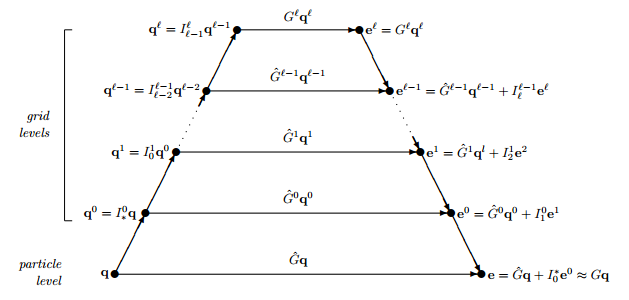
\includegraphics[width=0.8\textwidth]{levels.PNG}
\caption{Hierarchal decomposition of potential into two parts: close range interaction and smooth long-range interactions which can be approximated by an interpolation.\cite{3}}
\end{figure}

%--------------------------------------------
\section{Numerical Results}\label{sec:num}
The smoothing operation has been implemented for the solver to be used in the splitting. An example comparison of the pre/post-smoothing is shown in Figure 2.

Using the algorithm described above, a simple demonstration code was developed consisting of a fixed 3 level hierarchy: particle/coarse/coarsest grid. A cutoff radius was selected so that $a/h = 4$ to ensure sufficient accuracy, with the coarse and coarsest grids having $h=1/16$ and $h=1/8$ respectively. The values selected for $a$ and $h$ ensures reach of nearby grid charges on the coarsest grid covers the full domain. As an example of the reduction from the dense matrix $K$ of all pairwise interactions to a combination of sparse multilevel interactions, consider Figure 3 which shows the sparsity pattern of the nearby pairwise interactions at the particle level ($K0$).

A set of $n=1024$ particles with a Gaussian strength distribution was selected for the problem to study, with the Gaussian bump's width chosen so that it decays to within machine precision at the boundary of the domain. This ensures that minimal treatment is necessary for boundary considerations. Figure 4 compares plots of the electric potential for the exact pairwise ``naive'' method and the approximate MSM solution.

There are several features to note. First even the exact solution is not a perfect Gaussian, primarily because the particles are randomly distributed across the domain and there are comparatively few of them. The MSM solution manages to recover some of these fluctuations, but not all. Additionally the MSM solution fails to properly converge to the exact solutions values near the boundary. This is not surprising given now explicit treatment of boundary conditions was attempted, and clearly in the exact solution the potential has not decayed to near machine precision at the boundary of the domain. This means the MSM grids should probably be extended beyond the extent of the proper domain to correctly include boundary details.

An attempt was not made to compare the relative cost of the full pairwise interactions with the MSM as the problem sized studied was too small to properly elicit noticeable scaling effects. In order to study larger problem sizes an alternative means for generating kernel values would be necessary to fit in a reasonable memory footprint.



\begin{figure}[!htb]
\centering
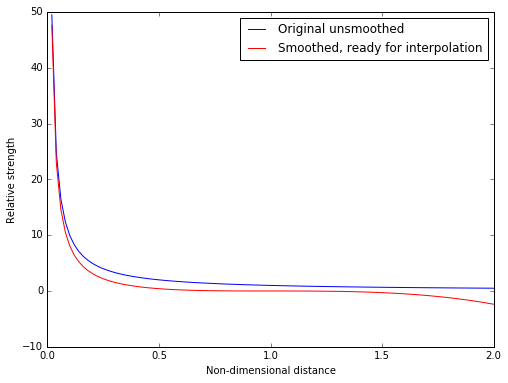
\includegraphics[width=0.6\textwidth]{smooth.PNG}
\caption{Comparison of original and smoothed interaction for a single particle.}
\end{figure}

\begin{figure}[!htb]
\centering
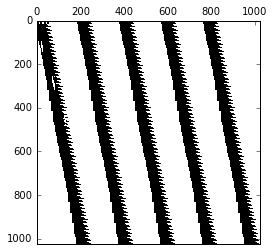
\includegraphics[width=0.4\textwidth]{K0.PNG}
\caption{Sparsity pattern of nearby particle pair-wise interactions with $r<a$ that form $K0$.}
\end{figure}

\begin{figure}[!htb]
\centering
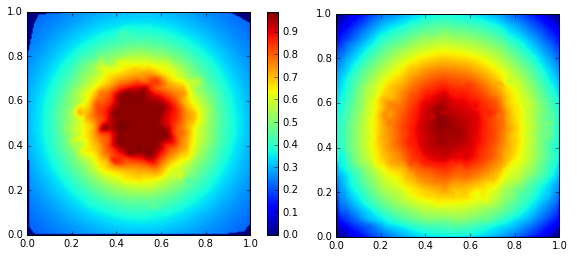
\includegraphics[width=1\textwidth]{UgComp.PNG}
\caption{Comparison of exact(left) and approximate MSM(right) potentials; Gaussian strength distribution, n=1024.}
\end{figure}

\newpage

%--------------------------------------------
\section{Conclusions}\label{sec:conc}
The multilevel summation method provides an alternate means of efficiently evaluating n-body problems. Also, in comparison to a FMM there are fewer components necessary for an efficient implementation. A simple MSM implementation was constructed and used to examine a simple test problem. The MSM solution managed to approximately replicate the exact solution. A more robust and fully capable MSM solver would have an adaptable number of grid levels so that the first grid interpolation level would more fully capture finer solution details.
%--------------------------------------------
\begin{thebibliography}{3}
\bibitem{1}
 David J. Hardy, Zhe Wu, James C. Phillips, John E. Stone, Robert D. Skeel, and Klaus Schulten. Multilevel Summation Method for Electrostatic Force Evaluation. Journal of Chemical Theory and Computation 2015 11 (2), 766-779 DOI: 10.1021/ct5009075
\bibitem{2}
Hardy, D. J. Multilevel summation for the fast evaluation of forces for the simulation of biomolecules. Ph.D. thesis, University of Illinois at Urbana−Champaign, Champaign, IL, 2006; Also Department of Computer Science Report No. UIUCDCS-R-2006-2546, May 2006.
\bibitem{3}
Bond, Stephen D. Multilevel summation methods for efficient evaluation of long-range pairwise interactions in atomistic and coarse-grained molecular simulation. No. SAND2014-0355. Sandia National Laboratories (SNL-NM), Albuquerque, NM (United States), 2014.
\bibitem{4}
Skeel, Robert D., Ismail Tezcan, and David J. Hardy. "Multiple grid methods for classical molecular dynamics." Journal of Computational Chemistry 23, no. 6 (2002): 673-684.

\end{thebibliography}

%--------------------------------------------
\clearpage
\appendix
\section{Code}
\newline
Apologies for formatting, source file width was a poor match for document width; rather than unnecessary line wrapping I have opted to reduce the font size. Original source file available upon request. 
\begin{lstlisting}[language=Python,basicstyle=\tiny]
#Multilevel summation method simple demonstration code with 2 grid level hierarchy
#Attempts to calculate electric potential for gaussian distribution of charges
import numpy as np
import scipy as sp
import scipy.interpolate as interp
import matplotlib.pyplot as plt

na = np.newaxis

n = 1024 #2**even
nh = int(np.sqrt(n)/2) #number of coarse grid squares on a side
A = 4/nh #cutoff length

px=np.array([]); py=px.copy() #Construct set of random bodies, roughly evenly
for i in np.arange(0,1,1/nh):
    for j in np.arange(0,1,1/nh):
        px = np.r_[px,i+np.random.rand(4)/nh]
        py = np.r_[py,j+np.random.rand(4)/nh]

pr = np.c_[px,py]

q = np.exp(-( (px-0.5)**2/(2*0.15**2) + (py-0.5)**2/(2*0.15**2) )) #Gaussian strength
#q = np.random.rand(n)

h = 16+2j #Coarse grid size
h_x, h_y = np.mgrid[0:1:h, 0:1:h] #coarse grid points
qh = interp.griddata(pr, 4*q, (h_x,h_y), method='cubic', fill_value=0) #interpolated coarse grid charges
Kh = np.sqrt((h_x.ravel()[:,na]-h_x.ravel())**2 + (h_y.ravel()[:,na]-h_y.ravel())**2) #interpolated coarse kernel values
np.fill_diagonal(Kh, 0) #remove self-influence

Uh = Kh@qh.ravel() #Calculate coarse grid potential contribution

#Repeat for coarsest grid
#Note that 2A is large enough to cover whole domain, even coarser grid would be a waste
h2 = 8+2j
h2_x, h2_y = np.mgrid[0:1:h2, 0:1:h2]
qh2 = interp.griddata(pr, 16*q, (h2_x,h2_y), method='cubic', fill_value=0)
Kh2 = np.sqrt((h2_x.ravel()[:,na]-h2_x.ravel())**2 + (h2_y.ravel()[:,na]-h2_y.ravel())**2)

Uh2 = Kh2@qh2.ravel()

Uh2qh = interp.griddata(np.c_[h2_x.ravel(),h2_y.ravel()], Uh2, (h_x,h_y), method='cubic', fill_value=0) #Coarsest grid onto coarse grid

#For simplicity generate full O(n^2) kernel for comparison, then construct MSM K0 from this
K = 1/np.sqrt((px[:,na]-px)**2 +(py[:,na]-py)**2)
np.fill_diagonal(K, 0)

#Select nearby exact kernel values for particle level computations
#In practice this would be very expensive, but for simplicity/demonstration it suffices
K0 = np.zeros([n,n])
for i in range(0,nh*4):
    for j in range(0,nh):
        #xs and ys are the coarse grid squares with A range of each target
        xs = i+(np.arange(-4,5)*nh*4-np.arange(4)[:,na])
        xs = xs[xs>=0]
        xs = xs[xs<n]
        ys = j+np.arange(-16,17)
        ys = ys[ys>=0]
        ys = ys[ys<n]
        xsm,ysm = np.meshgrid(xs,ys)
        K0[i*(nh)+j,xsm.ravel()*3+ysm.ravel()*2] = K[xsm.ravel(),ysm.ravel()]

U = K@q #Exact full pair-pair interactions for comparison
U0 = K0@q
a,b = np.mgrid[0:1:200j, 0:1:200j]
#Exact solution for potential, cap potential display maximums to a "good" value to minimize local clustering from dominating plot
Ug = interp.griddata(pr, np.minimum(U,np.mean(U)+2*np.std(U)), (a,b), method='cubic', fill_value=0)
#Interpolate particle, coarse grid, and coarsest grid particle values to a grid for easier plotting
Ug0 = interp.griddata(pr, U0, (a,b), method='cubic', fill_value=0)
Ug1 = interp.griddata(np.c_[h_x.ravel(),h_y.ravel()], Uh.ravel(), (a,b), method='cubic', fill_value=0)
Ug2 = interp.griddata(np.c_[h_x.ravel(),h_y.ravel()], Uh2qh.ravel(), (a,b), method='cubic', fill_value=0)

#MSM calculated values (scaled by a constant C and offset)
plt.imshow((Ug0/16-Ug1*2-Ug2*4), extent=(0,1,0,1),origin='lower')
plt.show()
#Pairwise exact calculated values
plt.imshow(Ug/1000, extent=(0,1,0,1),origin='lower')
plt.colorbar()
plt.show()

plt.spy(K0) #Sparsity pattern for nearby particle interactions at particle level, "kinda" sparse
\end{lstlisting}

\end{document}
